% Author: Zdeněk Lapeš <lapes.zdenek@gmail.com> (xlapes02)


\documentclass[a4paper, 11pt]{article}


%\usepackage[czech]{babel}
\usepackage[british,UKenglish,USenglish,english,american]{babel}
\usepackage[utf8]{inputenc}
\usepackage[left=2cm, top=3cm, text={17cm, 24cm}]{geometry}
\usepackage{times}
\usepackage{graphicx,wrapfig,lipsum}
\usepackage{float}
\usepackage[unicode]{hyperref}
\usepackage[usenames, dvipsnames]{color} % color
\usepackage{enumitem}
\usepackage{tabularx}
\usepackage{booktabs}
\usepackage{caption}
\usepackage{listings}

\graphicspath{ {images/} }
\hypersetup{
    colorlinks = true,
    hypertexnames = false,
    citecolor = red,
}


\begin{document}
    %%%%%%%%%%%%%%%%%%%%%%%%%%%%%%%% Titulní stránka %%%%%%%%%%%%%%%%%%%%%%%%%%%
    \begin{titlepage}
        \begin{center}
            
\includegraphics[width=0.77\linewidth]{FIT_logo} \\

            \vspace{\stretch{0.382}}

            \Huge{Project dokumentation} \\
            \LARGE{\textbf{
                ARM\-FITkit3 či jiný HW: Hra HAD
            }} \\
            \Large{IMP \- Microprocessors and Embedded Systems}

            \vspace{\stretch{0.618}}
        \end{center}

        {\Large
        \today
        \hfill
        Zdeněk Lapeš (xlapes02)

            \hfill
            \large{\textit{lapes.zdenek@gmail.com}}
        }
    \end{titlepage}


    %%%%%%%%%%%%%%%%%%%%%%%%%%%%%%%% Content %%%%%%%%%%%%%%%%%%%%%%%%%%%%%%%%%%%%%
    \pagenumbering{roman}
    \setcounter{page}{1}
    \tableofcontents
    \clearpage


    %%%%%%%%%%%%%%%%%%%%%%%%%%%%%%%% Setup First content page %%%%%%%%%%%%%%%%%%
    \pagenumbering{arabic}
    \setcounter{page}{1}


    %%%%%%%%%%%%%%%%%%%%%%%%%%%%%%%% Úvod %%%%%%%%%%%%%%%%%%%%%%%%%%%%%%%%%%%%%%


    \section{Introduction}\label{sec:introduction}
    The task was to create a Snake Game for the ARM\-FITkit3 board based on
    microcontroller Kinetis K60 (with ARM Cortex\-M4 core) and 2x matrix displays
    (type: KWM\-30881AGB, decoder: 74HCT154).

    The result is a Snake game written in C language using
    KDS IDE\cite{KDSIDE}.
    Snake is displayed on the matrix displays and the player can control
    the snake using the \textit{Fitkit3} 5 built\-in buttons.
    \newline

    %%%%%%%%%%%%%%%%%%%%%%%%%%%%%%%% Preparation %%%%%%%%%%%%%%%%%%%%%%%%%%%%%%%


    %%%%% Preparation %%%%%


    \section{Preparation}\label{sec:preparation}

    %%%%% Hardware %%%%%

    \subsection{Hardware}\label{subsec:hardware}
    The provided HW for this project is \textit{Fitkit3} board and one
    board with 2x matrix displays.
    The board with 2 matrix displays is connected to the
    \textit{Fitkit3} board using the connectors
        {\color{Green}{P1}} (placed on the Fitkit3 board) and connector
        {\color{Red}{P3}} (placed on the matrix display's board).
    One matrix display is (8,8) so the total size of the display is (16,8).

    \begin{figure}[h]
        \centering
        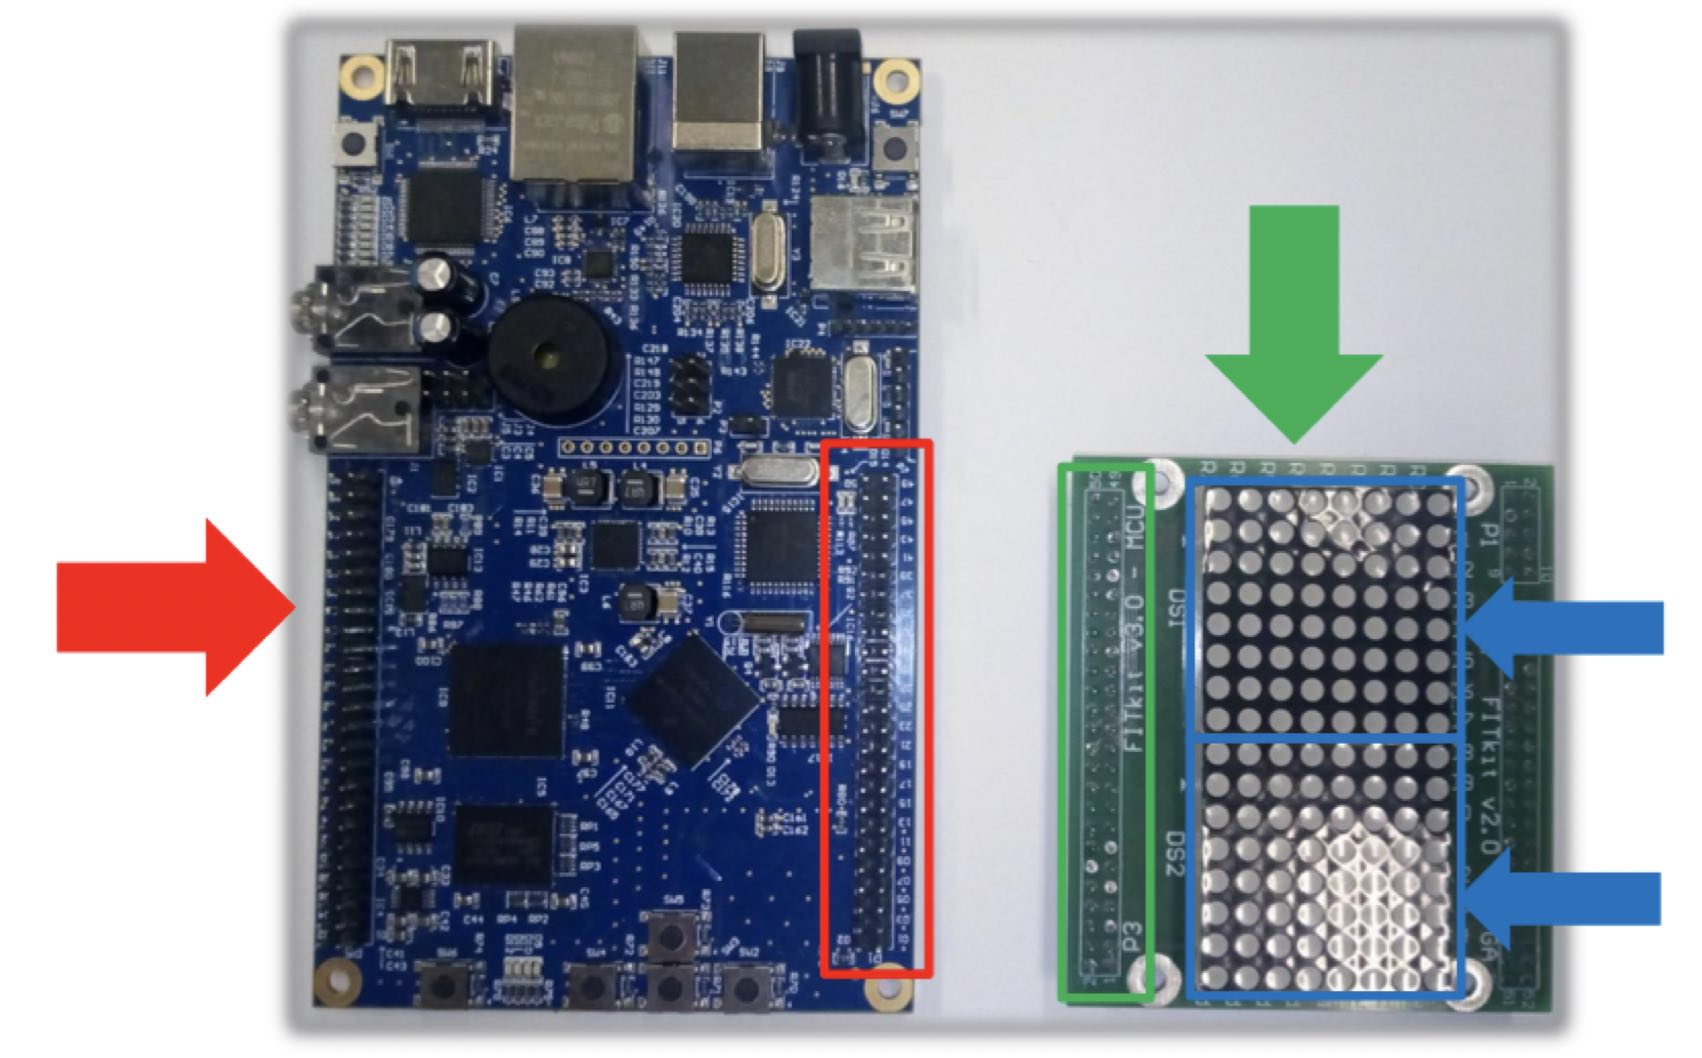
\includegraphics[width=0.75\textwidth]{equipments}
        \caption{Fitkit3 board \& matrix display board}\label{fig:figure1}
    \end{figure}


    %%%%%%%%%%%%%%%%%%%%%%%%%%%%%%%% Implementation %%%%%%%%%%%%%%%%%%%%%%%%%%%%


    \section{Implementation}\label{sec:implementation}
    Implementation of the game is inside file: \texttt{Sources/main.c}.
    All other files were created by the KDS IDE for MCU K60.

    The entry point of the program is the function \texttt{main()} located in
    \texttt{Source/main.c} file.
    At the beginning of the program, the function \texttt{SystemConfig()} is called
    where the peripherals of MCU are configured:
    \begin{itemize}
        \item Configuration of PTA's pins (GPIO) for the matrix displays.
        \item Configuration of PTE's pins (GPIO) for the buttons.
        \item Configuration of PIT (used for timer).
        \item Timer and Button interrupts are enabled.
    \end{itemize}

    After MCU configiration is \texttt{snake\_t} structure is initialized.
    This structure contains all information about the snake:
    \textbf{body}, \textbf{direction}, \textbf{speed}.

    Then the game starts
    by continue to endless loop, where all incoming interrupts
    by \textbf{PIT} timer and buttons are handled, using the functions
    \texttt{PIT0\_IRQHandler()} and \texttt{PORTE\_IRQHandler()}.

    \subsection{Timer interrupt Handler:}
    Snake next position is calculated here and display is
    updated by calling one of the functions:
    \texttt{move\_up()}, \texttt{move\_down()}, \texttt{move\_left()},
    \texttt{move\_right()}.

    \begin{lstlisting}[
        language=C,
        basicstyle=\small\ttfamily,
        keywordstyle=\color{blue},
        commentstyle=\color{green},
        tabsize=2
    ]
void PIT0_IRQHandler() {
    int column_number = i % 4;

    // Clear the timer's interrupt flag
    PIT->CHANNEL[0].TFLG = 0x1;

    // Set new snake body position
    if (snake.direction == RIGHT && TIMER_CHANGE_OFSET(i)) {
        move_right();
    } else if (snake.direction == UP && TIMER_CHANGE_OFSET(i)) {
        move_up();
    } else if (snake.direction == DOWN && TIMER_CHANGE_OFSET(i)) {
        move_down();
    } else if (snake.direction == LEFT && TIMER_CHANGE_OFSET(i)) {
        move_left();
    }

    // Place snake onto LED display
    ENABLE_LED_WRITE;
    if (column_number == 0) { PTA->PDOR = snake.head; }
    else if (column_number == 1) { PTA->PDOR = snake.body1; }
    else if (column_number == 2) { PTA->PDOR = snake.body2; }
    else if (column_number == 3) { PTA->PDOR = snake.tail; }
    DISABLE_LED_WRITE;

    //
    i++;
}
    \end{lstlisting}

    \subsection{Button interrupt Handler}
    Snake direction, speed and position is changed here according to the
    pressed button.\\


    \begin{lstlisting}[
        language=C,
        basicstyle=\small\ttfamily,
        keywordstyle=\color{blue},
        commentstyle=\color{green},
        tabsize=2
    ]
void PORTE_IRQHandler(void) {
    // Wobble
    if (IS_BTN_INTERRUPT_WOBBLE == 0) {
        // Clear interupt flags
        PORTE->ISFR = BTNs_ALL_MASK;
        return;
    }

    delay(tdelay1 / 100, 1); // Filtering wobble

    // BTN_DOWN
    if (IS_CLICK_DOWN && snake.direction == UP) {
        snake.direction = RIGHT;
    } else if (IS_CLICK_DOWN && snake.direction == DOWN) {
        snake.direction = LEFT;
    } else if (IS_CLICK_DOWN && snake.direction == LEFT) {
        snake.direction = UP;
    } else if (IS_CLICK_DOWN && snake.direction == RIGHT) {
        snake.direction = DOWN;
    }

    // BTN_UP
    if (IS_CLICK_UP && snake.direction == UP) {
        snake.direction = LEFT;
    } else if (IS_CLICK_UP && snake.direction == DOWN) {
        snake.direction = RIGHT;
    } else if (IS_CLICK_UP && snake.direction == LEFT) {
        snake.direction = DOWN;
    } else if (IS_CLICK_UP && snake.direction == RIGHT) {
        snake.direction = UP;
    }

    // Speed
    if (IS_CLICK_RIGHT && snake.speed > 50) {
        snake.speed -= 50;
    } else if (IS_CLICK_LEFT && snake.speed < 350) {
        snake.speed += 50;
    }

    // Restart game
    if (IS_CLICK_START_STOP) {
        init_snake_body_variables();
    }

    // Clear interupt flags
    PORTE->ISFR = BTNs_ALL_MASK;
}
    \end{lstlisting}



    %%%%%%%%%%%%%%%%%%%%%%%%%%%%%%%% FUNCTIONALITY %%%%%%%%%%%%%%%%%%%%%%%%%%%%

    %%%%% Button interrupt handling %%%%%


    \section{Functionality \& Game Control}\label{sec:functionality}

    \subsection{About the Game}\label{subsec:functionality-of-the-game}
    The game is a single player game.

    \subsubsection{Game Control}\label{sbsubsec:controling}
    The game is controlled by the \textit{Fitkit3} built\-in buttons:
    \begin{itemize}
        \item \textbf{SW2} \- Snake speed up.
        \item \textbf{SW3} \- Snake turn right.
        \item \textbf{SW4} \- Snake speed down.
        \item \textbf{SW5} \- Snake turn left.
        \item \textbf{SW6} \- Snake reset (default speed and starting position).
    \end{itemize}

    \begin{figure}[H]
        \centering
        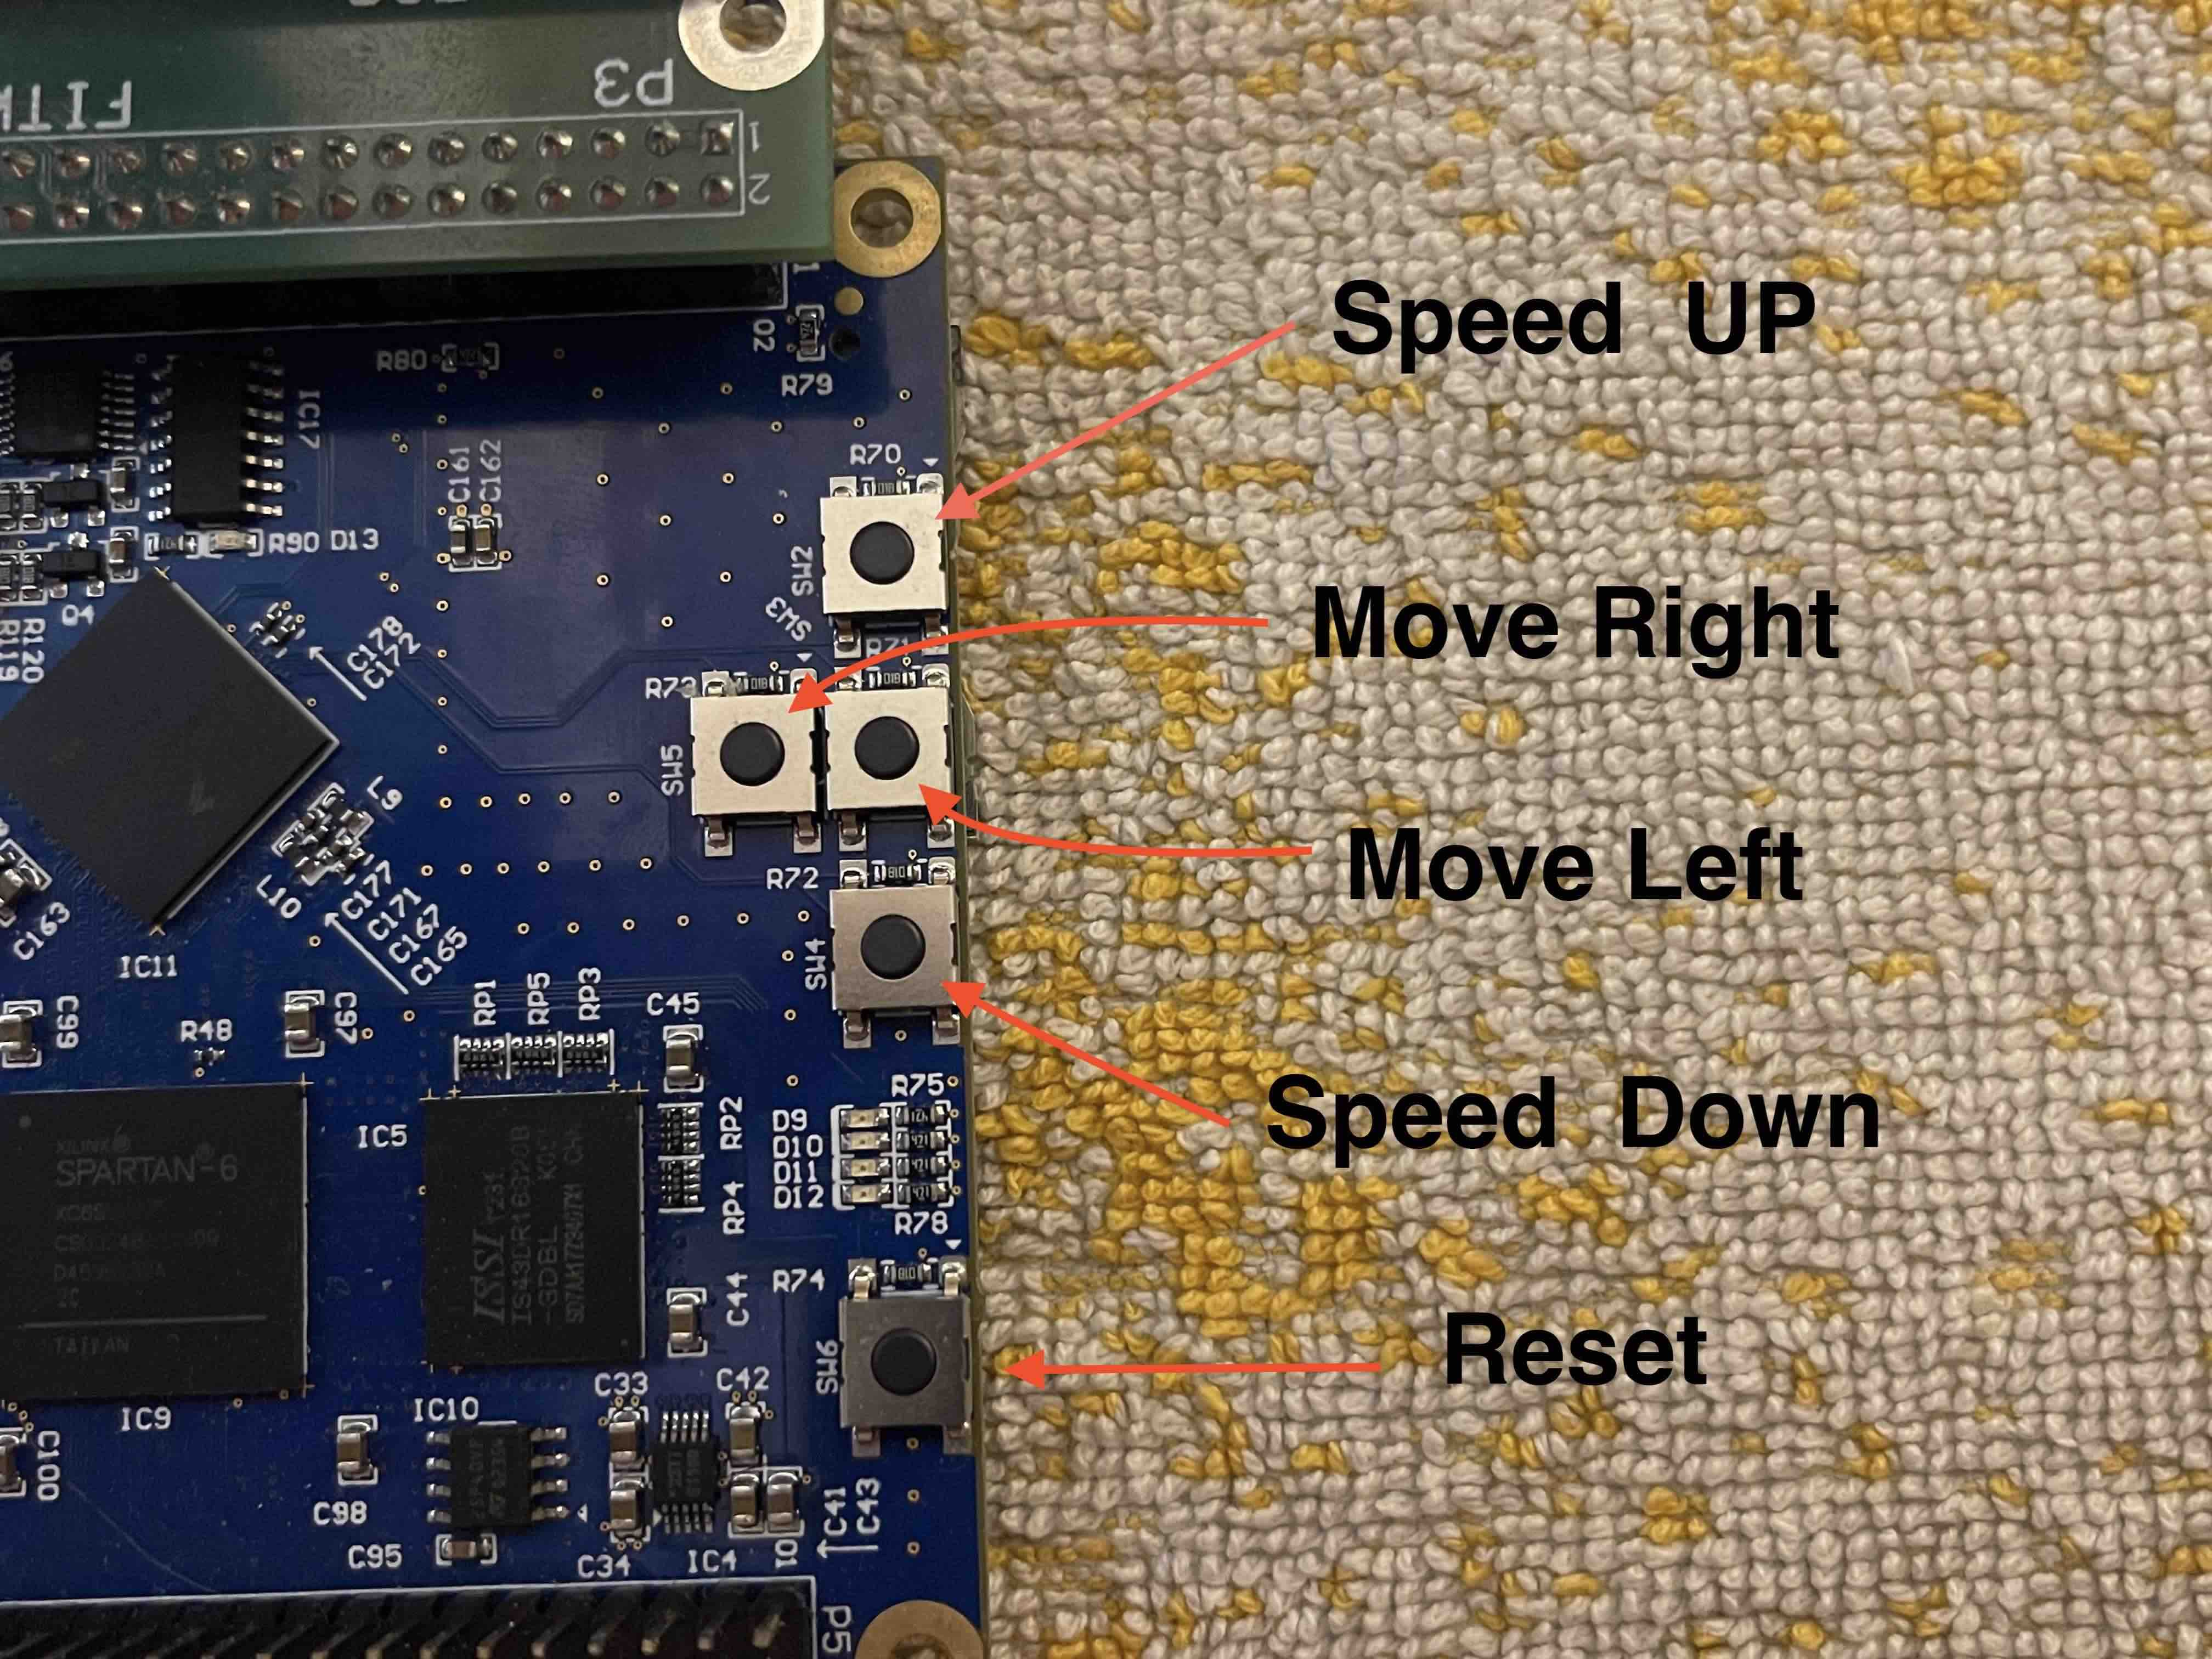
\includegraphics[width=0.5\textwidth]{buttons}
        \caption{Fitkit3 Buttons}\label{fig:figure2}
    \end{figure}

    The Snake starts moving to the right with normal speed
    at the beginning of the game.
    By pressing the coressponding button, you can change the snake speed and direction.
    If you want reset the game, press the button \textbf{SW6}, which sets
    the speed to the default value and places snake to the starting position.

    \section{Demonstration of implemented game}\label{sec:demonstration}
    The game is demonstrated in the video on this url: \textbf{https://youtu.be/V0ONHRM66mM}.

    %%%%%%%%%%%%%%%%%%%%%%%%%%%%%%%% Conclusion %%%%%%%%%%%%%%%%%%%%%%%%%%%%%%%%


    \section{Conclusion}\label{sec:conclusion}
    The project was successfully completed and the game is working as expected.
    I managed to implement whole functionality of the game with some additional
    features like speed up/down and reset\ref{sbsubsec:controling}.
    In project I used the timer interrupt for controlling the snake moves
    and button interrupts for controlling the snake direction and speed.


    %%%%%%%%%%%%%%%%%%%%%%%%%%%%%%%% Autoevaluation %%%%%%%%%%%%%%%%%%%%%%%%%%%%%%%%


    \section{Autoevaluation}\label{sec:autoevaluation}
    \begin{table}[H]
        \centering
        \caption{Autoevaluation}\label{tab:table1}
        \label{tab:my_label}
        \begin{tabularx}{\textwidth}{XXX}
            \toprule
            \textbf{Task}  & \textbf{Points} & \textbf{Description}                                                                                                      \\
            \midrule
            \textbf{E}     & 1               & I began long before the deadline and afterward I needed to fix some special cases, what I have learned from laboratories. \\
            \hline
            \textbf{F}     & 5               & The whole functionality requirements were covered.                                                                        \\
            \hline
            \textbf{Q}     & 3               & Code should be straightforward to understand almost everybody.                                                            \\
            \hline
            \textbf{P}     & 1               & Illustration of functionality can be watched on youtube \href{https://youtu.be/V0ONHRM66mM}{click here to watch}          \\
            \hline
            \textbf{D}     & 4               & All documentation requirements are covered.                                                                               \\
            \hline
            \textbf{Total} & 14              &                                                                                                                           \\
            \bottomrule
        \end{tabularx}

    \end{table}


    %%%%%%%%%%%%%%%%%%%%%%%%%%%%%%%% Citace %%%%%%%%%%%%%%%%%%%%%%%%%%%%%%%%%%%%
    \clearpage
    \bibliographystyle{bst/czechiso}
    \renewcommand{\refname}{Literature}\label{sec:literatura}
    \bibliography{manual}


\end{document}
